\documentclass{beamer}
\usepackage[utf8]{inputenc}
\usepackage{hyperref}
\usepackage[scaled]{beramono}
\usepackage[T1]{fontenc}
\usepackage{listings}
\usepackage{graphicx}
\usepackage{tabularx}
\usepackage{multicol}
\usepackage{tikz}
\usepackage{pgfplots}
\usepackage{multicol}

\graphicspath{{.images/}}

\definecolor{gray1}{rgb}{0.9,0.9,0.9}



\lstset{backgroundcolor=\color{gray1},frame=single,framerule=0pt,language=C,basicstyle=\small}

\usetheme[compress]{Dresden}
\usecolortheme{beaver}

\setbeamertemplate{itemize item}{\textbullet}
\setbeamertemplate{navigation symbols}{}
\defbeamertemplate*{footline}{shadow theme}
{%
  \leavevmode%
  \hbox{\begin{beamercolorbox}[ht=2.5ex,dp=1.125ex,leftskip=.3cm plus1fil,rightskip=.3cm]{author in head/foot}%
    \usebeamerfont{author in head/foot}\insertshortauthor\hfill\insertshorttitle\hfill\insertframenumber\,/\,\inserttotalframenumber
  \end{beamercolorbox}}%
  \vskip0pt%
}



%---------------------------------------------------
% CONTENT
%---------------------------------------------------

\title{Isilon Solutions + OneFS}
\author{Anne-Victoria Meyer}
\institute{Universität Hamburg}
\date{Proseminar »Ein-/Ausgabe – Stand der Wissenschaft«, 2013}
\subject{Informatik}



\begin{document}


%\subsection{}
\frame{\titlepage}

%\subsection{}
\begin{frame}
  \frametitle{Inhalt}
  \setcounter{tocdepth}{1}
  \setbeamertemplate{section in toc}[sections numbered]
  \tableofcontents
\end{frame}


\section{Einleitung}

\subsection{EMC Isilon}
\begin{frame}[fragile]
  \frametitle{EMC Isilon}
  %\begin{itemize} 
  %\end{itemize}
  \begin{description}
    \item[2001] Gründung als \emph{Isilon Systems}
    \item[2010] aufgekauft von \emph{EMC Corporation}
    \item[] 
    \item[Produkt]Speicherlösungen
    \item[Kunden]große Unternehmen
    \item[Technologie]Scale-Out-NAS\footnote{Network Attached Storage}          
  \end{description}

\end{frame}

\subsection{}
\begin{frame}[fragile]
  \frametitle{EMC Isilon}
\begin{description}         
    \item[Leitwerte] $\rightarrow$ Einfachheit
    \item $\rightarrow$ Skalierbarkeit
    \item $\rightarrow$ Performance
    \item[]
    \item[Beispiele] $\rightarrow$ \emph{Lightstorm Entertainment} nutzte Speicherlösungen von Isilon für die Produktion des Filmes \emph{Avatar}
    \item $\rightarrow$ \emph{Apple} nutzt u.A. Speicherlösungen von Isilon für den \emph{iTunes Store}
  \end{description}

\end{frame}

\subsection{}
\begin{frame}[fragile]
  \frametitle{Network Attached Storage}
  \begin{center}\includegraphics[width=0.8\textwidth]{nas.pdf}\end{center}
\end{frame}

\subsection{}
\begin{frame}[fragile]
  \frametitle{Hardwareaufbau}
  
  \begin{figure}[htp]
    \centering
    \includegraphics[width=0.7\textwidth]{onefs-neu.pdf}
  \end{figure}

\end{frame}


\subsection{}
\begin{frame}[fragile]
  \frametitle{Schichten}
  
  \begin{figure}[htp]
    \centering
    \includegraphics[width=0.8\textwidth]{conclusion.pdf}
    \caption{[EMC Corp. 2012]}
  \end{figure}

\end{frame}

\section{Hardware}

\subsection{}

  \begin{frame}[fragile]
  \frametitle{Nodes}
  
  \begin{figure}[htp]
    \centering
    \includegraphics[width=0.7\textwidth]{isilon-family.jpg}
    \caption{[EMC Corp. 2012]}
  \end{figure}
  
  \vspace{-5mm}
  
  \begin{itemize}
    \item Während Onlinebetrieb erweiterbar
    \item Nodes aller Reihen in einem Dateisystem vereinbar \\
    zu virtuellem Volume 
    \vspace{1mm}
    \item[$\rightarrow$] \textbf{Flexibilität}
    \end{itemize}

\end{frame}

\subsection{}


\begin{frame}[fragile]
  \frametitle{S-Serie}
  
  \begin{figure}[htp]
    \centering
    \includegraphics[width=0.8\textwidth]{isilon-s.jpg}
    \caption{[EMC Corp. 2012]}
  \end{figure}
  
    \begin{description} 
    \item[Verwendung] für IOPS-intensive Prozesse 
    \vspace{5mm}
    \item[Kapazität]300, 600 oder 900GB HDDs
    \item[Anzahl] 24 HDDs pro Node 
    \item[alternativ] bis zu 6 HDDs durch SSDs austauschbar
        
  \end{description}

\end{frame}

\subsection{}
\begin{frame}[fragile]
  \frametitle{X-Serie}
  
  \begin{figure}[htp]
    \centering
    \includegraphics[width=0.8\textwidth]{isilon-x.jpg}
    \caption{[EMC Corp. 2012]}
  \end{figure}
  
  \begin{description} 
    \item[Verwendung] vielfältig einsetzbar 
    \vspace{5mm}
    \item[Kapazität] von 500GB bis 4TB HDDs möglich
    \item[Anzahl]  12 oder 36 HDDs pro Node 
    \item[alternativ] bis zu 6 HDDs durch SSDs austauschbar
        
  \end{description}

\end{frame}

\subsection{}
\begin{frame}[fragile]
  \frametitle{NL-Serie}
  
  \begin{figure}[htp]
    \centering
    \includegraphics[width=0.8\textwidth]{isilon-nl.jpg}
    \caption{[EMC Corp. 2012]}
  \end{figure}
  
  \begin{description} 
    \item[Verwendung] Langzeitspeicherung / Archivierung
    \vspace{5mm}
    \item[Kapazität] 1, 2, 3 oder 4TB HDDs
    \item[] 36 HDDs pro Node 
        
  \end{description}

\end{frame}

\subsection{}
\begin{frame}[fragile]
  \frametitle{Extension Nodes}
  \begin{figure}[htp]
    \centering
    \includegraphics[width=0.5\textwidth]{isilon-pa.jpg}
    \caption{[EMC Corp. 2013]}
  \end{figure}
  
  \begin{description}
    \item[Performance Accelerator] erhöht Datendurchsatz im Cluster
    \item[Backup Accelerator] Zuständig für Datensicherung
  \end{description}

  
\end{frame}

\section{OneFS}

\subsection{}
\begin{frame}[fragile]
  \frametitle{Hardwareaufbau und OneFS}

  \begin{center}\includegraphics[width=0.7\textwidth]{onefs-neu.pdf}\end{center}

\end{frame}  

\subsection{}
\begin{frame}[fragile]
  \frametitle{Sicht der Clients}

  \begin{center}\includegraphics[width=0.7\textwidth]{onefs2-neu.pdf}\end{center}

\end{frame}  

\subsection{}
\begin{frame}[fragile]
  \frametitle{OneFS (OS)}

  \begin{description}
    \item[Kernel] freeBSD
    \item[Shell] Z Shell (zsh) + 'isi'-Befehle
    \item[Version] 7.0
    \item[Protokolle] NFS, SMB/CIFS (default)
    \item[] (HTTP, FTP, HDFS, iSCSI, REST API) 

   \end{description}

\end{frame}    

\subsection{}
\begin{frame}[fragile]
  \frametitle{OneFS (Dateisystem)}

  \begin{description}
    \item[B-Trees] effiziente Suche
    \item[Adressierung] \{Node, Platte, Offset\}
    \item[Journaling] im NVRAM (Non-Volatile Random Access Memory)
    \item[Striping] erst über alle Nodes, dann ggf. über \\Festplatten innerhalb der Nodes
    \item[Sicherung] Paritäten, Mirroring individuell einstellbar
    \item[Metadaten] Speicherung in Inodes, häufig auf SSDs, um Performance zu erhöhen
  \end{description}

\end{frame}

\subsection{}
\begin{frame}[fragile]
  \frametitle{OneFS (Dateisystem) - Das Schreiben einer Datei}
  
  \begin{enumerate}
    \item Client sendet Schreibanfrage an Node A (Front-End-Netzwerk)
    \item Node A legt Striping und Sicherung fest
    \item Node A schreibt einen Block in den eigenen Speicher,
    verteilt die weiteren Blöcke auf andere Nodes (Back-End-Netzwerk)
    \end{enumerate}
  
  \begin{itemize}
    \item Daten werden vorerst in NVRAM geschrieben 
    \item Administrator kann optional aus drei Layouts wählen, \\
    je nach Zugriffsmuster:
    \vspace{2mm}
    \item[$\rightarrow$] Nebenläufigkeit 
    \item[$\rightarrow$] Streaming
    \item[$\rightarrow$] Zufall
        
  \end{itemize}
  
  

\end{frame}

      

\subsection{}
\begin{frame}[fragile]
  \frametitle{Administration}
  
  \begin{figure}[htp]
    \centering
    \includegraphics[width=0.6\textwidth]{insightiq.jpg}
    \caption{[vFokus.no 2012]}
  \end{figure}
  
  \vspace{-5mm}

  \begin{itemize}
    \item WebUI
    \item CLI via SSH oder RS232 serieller Verbindung
    \item LCD Display an Nodes für Add/Remove-Funktionen
    \item RESTful Platform API
  \end{itemize}

\end{frame}  

\subsection{}
\begin{frame}[fragile]
  \frametitle{Tools}

  \begin{description}
    \item[InsightIQ] Performance Monitoring
    \item[SmartPools] Optimierung der Datenverteilung
    \item[SmartQuotas] Quota Management
    \item[SmartConnect] Lastverteilung und Failover
    \item[SnapshotIQ] Backup
    \item[Isilon for vCenter] Steuerung durch vCenter
    \item[SyncIQ] Datenvervielfältigung
    \item[SmartLock] Datenbewahrung
    \item[Aspera for Isilon] Isilon im Wide Area Network (WAN)
  \end{description}

\end{frame}    

\subsection{}
\begin{frame}[fragile]
  \frametitle{SmartConnect}
  
  \begin{figure}[htp]
    \centering
    \includegraphics[width=0.9\textwidth]{smartconnect-image.png}
    \caption{[EMC Corp. 2011]}
  \end{figure}

  \begin{itemize}
    \item[] 
  \end{itemize}

\end{frame}    

\subsection{}
\begin{frame}[fragile]
  \frametitle{Lastverteilung}

  \begin{itemize}
    \item[] SmartConnect \emph{Basic} wird mit OneFS mitgeliefert \\ SmartConnect \emph{Advanced} muss bei Bedarf erworben werden
  \end{itemize}
  
  \vspace{3mm}
  
  \begin{description}
    \item[Basic] DNS Round Robin
    \vspace{3mm}
    \item[Advanced] CPU Auslastung
    \item[] Verbindungsanzahl
    \item[] Durchsatz 
    \vspace{3mm}
    \item[] Failover und Failback
  \end{description}

\end{frame}  

\section{Benchmarks}

\subsection{}
\begin{frame}[fragile]
  \frametitle{Benchmarks CIFS}

  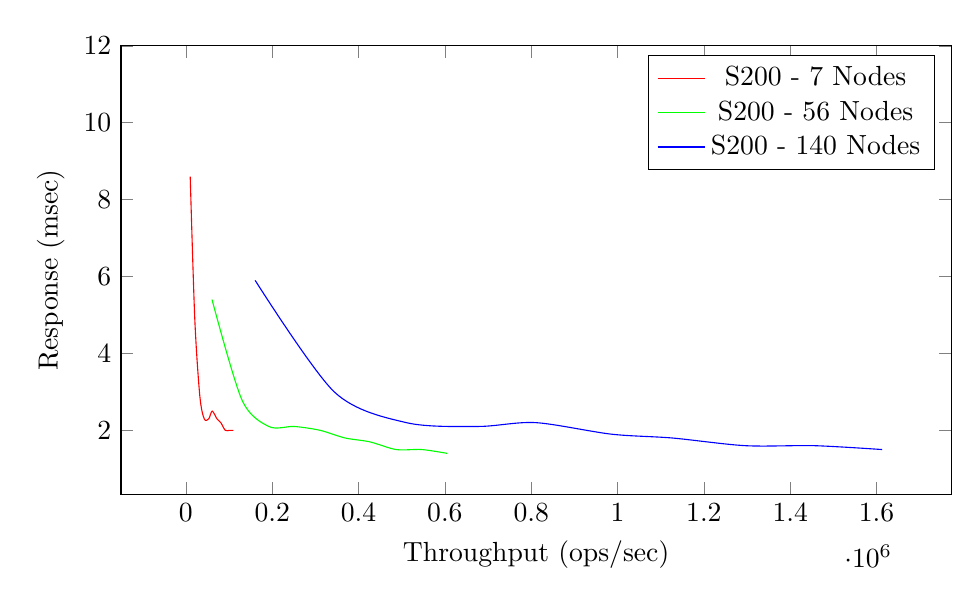
\begin{tikzpicture}
  \begin{axis}
  [
    xlabel=Throughput (ops/sec),
    ylabel=Response (msec),
    ymax=12,
    width=\textwidth,
    height=0.6\textwidth
  ]
  \addlegendentry{S200 - 7 Nodes}
  \addplot[smooth,mark=,red] plot coordinates
  {
    
    (10030,8.6)
    (20619,4.9)
    (32242,2.9)
    (42426,2.3)
    (53062,2.3)
    (60953,2.5)
    (71984,2.3)
    (80840,2.2)
    (91271,2.0)
    (100968,2.0)
    (110201,2.0)
  };
  \addlegendentry{S200 - 56 Nodes}
  \addplot[smooth,mark=,green] plot coordinates
  {
    (60534,5.4)
    (129503,2.8)
    (192153,2.1)
    (250999,2.1)
    (310806,2.0)
    (369024,1.8)
    (426202,1.7)
    (487029,1.5)
    (546452,1.5)
    (605629,1.4)
  };
  \addlegendentry{S200 - 140 Nodes}
  \addplot[smooth,mark=,blue] plot coordinates
  {
    (160444,5.9)
    (343685,3.0)
    (510558,2.2)
    (676766,2.1)
    (810117,2.2)
    (985376,1.9)
    (1126697,1.8)
    (1296466,1.6)
    (1456779,1.6)
    (1612778,1.5)
  };

  \end{axis}
  \end{tikzpicture}


\end{frame}

\section{Zusammenfassung}

\subsection{}
\begin{frame}[fragile]
  \frametitle{Zusammenfassung}

  \begin{multicols}{2}

    \begin{itemize}
      \item Scale-Out-NAS für Enterprise-Bereich
      \item Schwerpunkt: Einfachheit, Skalierbarkeit
      \item effiziente Implementierung
      \item Transparenz, globaler Namespace
      \item geringer Administrationsaufwand
    \end{itemize}

    \begin{figure}[htp]
    \centering
    \includegraphics[width=0.5\textwidth]{conclusion.pdf}
    \caption{[EMC Corp. 2012]}
  \end{figure}

  \end{multicols}

\end{frame}    

\subsection{}
\begin{frame}[fragile]
  \frametitle{Quellen (alle zuletzt abgerufen am 07.06.2013)}

  \tiny
  \begin{itemize}
    \item http://www.santutorial.com/?cat=11
    \item http://www.mitwa.org/node/8321
    \item http://arstechnica.com/business/2011/05/isilon-overview/
    \item http://www.enterprisestorageforum.com/storage-hardware/emc-isilon-buyers-guide.html
    \item http://www.hamburgnet.de/products/isilon.html?gclid=CPTLo7\_Ew7cCFajKtAodyxQAhQ
    \item http://www.scribd.com/doc/131726467/Onefs-Command-Ref-6-5
    \item http://www.ndm.net/emcstore/isilon/emc-isilon-s-series-platform-node
    \item http://www.ndm.net/emcstore/isilon/emc-isilon-x-series-platform-node
    \item http://www.ndm.net/emcstore/isilon/emc-isilon-nl-series-platform-node
    \item http://www.storagenewsletter.com/news/business/isilon-iq-lightstorm-entertainment
    \item http://www.emc.com/storage/isilon/isilon.htm 
    \item http://www.layer47.com/downloads/isilon\_whitepaper\_smartconnect.pdf
    \item http://www.emc.com/collateral/hardware/white-papers/h10719-isilon-onefs-technical-overview-wp.pdf
    \item http://www.emc.com/collateral/hardware/specification-sheet/h10690-ss-isilon-s-series.pdf
    \item http://www.emc.com/collateral/software/specification-sheet/h10639-isilon-x-series-ss.pdf
    \item http://www.emc.com/collateral/software/specification-sheet/h10640-isilon-nl-series-ss.pdf
    \item http://www.emc.com/collateral/data-sheet/h11231-ss-isilon-perf-acc.pdf
    \item http://www.emc.com/collateral/hardware/specification-sheet/h10791-isilon-backup-accelerator-ss.pdf
    \item http://www.emc.com/collateral/software/technical-documentation/h10689-cm-isd-3rdparty-sw.pdf
    
  \end{itemize}

\end{frame}

\subsection{}
\begin{frame}[fragile]
  \frametitle{Bildquellen}

  \tiny
  \begin{itemize}
    \item[\textbf{Foliennr.}] \textbf{Quelle}
    \item[7] "EMC Isilon scale-out storage solutions, powered by the OneFS operating system, provide users with a broad range of options to meet their specific storage needs." http://www.emc.com/collateral/software/data-sheet/h10541-isilon-scale-out-storage-platform-ds.pdf
    \item[8] "EMC Isilon Family Fanout" http://farm9.staticflickr.com/8246/8640896526\_31b5274651\_o.jpg
    \item[9] "EMC Isilon S-Series S200" http://farm9.staticflickr.com/8114/8639792225\_580efbb693\_o.jpg
    \item[10] "EMC Isilon X-Series X200" http://farm9.staticflickr.com/8395/8640895382\_08f6319600\_o.jpg
    \item[11] "EMC Isilon NL-Series NL200" http://farm9.staticflickr.com/8379/8639792473\_3f76bd3c2d\_o.jpg 
    \item[12] "EMC Isilon Performance Accelerator" http://www.emc.com/R1/images/EMC\_Image\_C\_1310616693624\_detail-image-emc-isilon-accelerator-shdw-front-300.jpg
    \item[18] (ohne Titel) http://vfokus.no/wp-content/uploads/2012/08/IQ.png
    \item[20] (ohne Titel) http://www.layer47.com/downloads/isilon\_whitepaper\_smartconnect.pdf
    \item[22] Grafik basierend auf Messergebnissen von:
    \item[] http://www.spec.org/sfs2008/results/res2011q2/sfs2008-20110527-00194.html
    \item[] http://www.spec.org/sfs2008/results/res2011q2/sfs2008-20110527-00188.html
    \item[] http://www.spec.org/sfs2008/results/res2011q2/sfs2008-20110527-00185.html
    \item[23] "EMC Isilon scale-out storage solutions, powered by the OneFS operating system, provide users with a broad range of options to meet their specific storage needs." http://www.emc.com/collateral/software/data-sheet/h10541-isilon-scale-out-storage-platform-ds.pdf 
  \end{itemize}
  
\end{frame}

\end{document}
